\documentclass{article}
\usepackage{amsmath}
\begin{document}

\title{My First LaTeX Document}
\author{Your Name}
\date{\today}
\maketitle

\section{Introduction}

\section{Theory}
\subsection{Discretization methods and finite differences}
For the analysis of partial differential equations (PDEs) and ordinary differential equations(ODEs)
numerical methods have shown to be a strong tool for the analysis of them. Among the different methods
there exist the finite difference methods, on which the space is discretized on grid points,
and the derivate are approximated with finite differences approximations. In a discretized space, with equidistant
points at $h$ distance we obtain:


\begin{enumerate}
    \item First order methods:
          \begin{itemize}
              \item Forward first order differences:
                    \begin{equation}
                        \frac{df(x_{i})}{dx} \approx \frac{f(x_{i+1}) - f(x_{i})}{h}
                    \end{equation}
              \item Backward first order differences:
                    \begin{equation}
                        \frac{df(x_{i})}{dx} \approx \frac{f(x_i) - f(x_{i-1})}{h}
                    \end{equation}
              \item Centered first order differences:
                    \begin{equation}
                        \frac{df(x_{i})}{dx} \approx \frac{f(x_{i+1}) - f(x_{i-1})}{h}
                    \end{equation}
          \end{itemize}

    \item Second order methods:
          \begin{itemize}
              \item Forward second order differences:
                    \begin{equation}
                        \frac{d^{2} f(x_{i})}{dx^2} \approx \frac{f(x_{i+2}) - 2f(x_{i+1}) + f(x_i)}{h^2}
                    \end{equation}
              \item Backward second order differences:
                    \begin{equation}
                        \frac{d^{2} f(x_{i})}{dx^2} \approx \frac{f(x_i) - 2f(x_{i-1}) + f(x_{i-2})}{h^2}
                    \end{equation}
              \item Centered second order differences:
                    \begin{equation}
                        \frac{d^{2} f(x_{i})}{dx^2} \approx \frac{f(x_{i+1}) - 2f(x_i) + f(x_{i-1})}{h^2}
                    \end{equation}
          \end{itemize}
\end{enumerate}
Where $i$ represent the position in space of the points ($x_{i} = h*i$).

\subsection{The wave equation}
Thw wave equation is a a partial deferential equation which describes the movement of waves, which cna be transpoort of voltage
lossless transmission line. Among it possible dimension equation,
in this project we describe the one dimensional wave-equation.

\begin{equation}
    \frac{d^{2} \psi}{dt^2} = c^{2} \cdot \frac{d^{2} \psi}{dx^2}
\end{equation}

On which, $\psi(x,t)$ is the the vibration amplitude, $c$ is $1/v$ of spread of the wave.

\subsection{The time Dependent Diffusion equation}
\section{Methods}

\subsection{The wave equation: Discretization and Simulation}
\subsubsection{The wave equation: Discretization}
For the evaluation of the wave equation,the space is discretized in $N$ points $x$ evenly spaced by $L/N = h$ on the one dimensional space ($L$ is length os string) a in $\tau$ in the temporal space.
Then, with centered second order differences, the wave equation second order terms are discretized in:
\begin{equation}
    \begin{aligned}
        \frac{d^{2} \psi}{dt^2} \approx \frac{\psi(x_{i},t_{m+1}) - 2\psi(x_i,t_{m}) + \psi(x_{i},t_{m-1})}{^2} \\
        \frac{d^{2} \psi}{dx^2} \approx \frac{\psi(x_{i+1},t_{m}) - 2\psi(x_i,t_{m}) + \psi(x_{i-1},t_{m})}{h^2}
    \end{aligned}
\end{equation}
Inserting on equation INSERTAR REFERENCIA and developing, the position/amplitude of the string in $x$ the next time step ($t= m+1$)
is defined as:
\begin{equation}
    \begin{aligned}
        \frac{\psi(x_{i},t_{m+1}) - 2\psi(x_i,t_{m}) + \psi(x_{i},t_{m-1})}{\tau^2} =
        c^{2} \cdot \frac{\psi(x_{i+1},t_{m}) - 2\psi(x_i,t_{m}) + \psi(x_{i-1},t_{m})}{h^2}                                                                         \\
        \psi(x_{i},t_{m+1}) = 2\psi(x_i,t_{m}) - \psi(x_{i},t_{m-1}) + c^{2} \tau^{2} \cdot \frac{\psi(x_{i+1},t_{m}) - 2\psi(x_i,t_{m}) + \psi(x_{i-1},t_{m})}{h^2} \\
        \psi(x_{i},t_{m+1}) = \psi(x_{i+1},t_{m})\tau^{2}\frac{c^{2}}{h^2} + 2\psi(x_i,t_{m}) \cdot (1 - \tau^{2}\frac{c^{2}}{h^2})  + \psi(x_{i-1},t_{m})\tau^{2}\frac{c^{2}}{h^2} -  \psi(x_{i},t_{m-1})
    \end{aligned}
\end{equation}

Note that equation INSERTAR REFERENCIA, can be transformed in matrix operation for the whole grid as $\mathbf{x}^{m+1}= \mathbf{A} \cdot \mathbf{x}^{m} - \mathbf{x}^{m-1}$, where $\mathbf{x}$ is the vector
with $\psi$ of the all the grid points. Thus, the tri-diagonal time-stepping matrix $\mathbf{A(c,\tau,h)}$ is:
\[
    \begin{bmatrix}
        2(1 - \tau^{2}\frac{c^{2}}{h^2}) & \tau^{2}\frac{c^{2}}{h^2} & 0      & \cdots                    & 0                                \\
        \tau^{2}\frac{c^{2}}{h^2}        & \ddots                    & \ddots & \ddots                    & \vdots                           \\
        0                                & \ddots                    & \ddots & \ddots                    & 0                                \\
        \vdots                           & \ddots                    & \ddots & \ddots                    & \tau^{2}\frac{c^{2}}{h^2}        \\
        0                                & \cdots                    & 0      & \tau^{2}\frac{c^{2}}{h^2} & 2(1 - \tau^{2}\frac{c^{2}}{h^2}) \\
    \end{bmatrix}
\]

\subsubsection{The wave equation: Simulation}
The simulation of the wave equation is done using the time stepping scheme  $\mathbf{x}^{m+1}= \mathbf{A} \cdot \mathbf{x}^{m} - \mathbf{x}^{m-1}$, with $L=1$,$c=1$ and $\tau = 0.001$.
In all simulations, the there are dirichlet boundary conditions ($\psi(x = 0,t) = \psi(x = L,t_{m}) = 0$) and the initial conditions ()$\psi(x,t = 0)$) are changed between:
\begin{enumerate}
    \item $\psi(x,t = 0) = sin(2\pi x)$.
    \item $\psi(x,t = 0) = sin(5\pi x)$.
    \item $\psi(x,t = 0) = sin(5\pi x)$ if $\frac{1}{5} < x < \frac{2}{5}$, else $\psi(x,t = 0) = 0$.
\end{enumerate}

\subsection{The time dependent diffusion equation: Discretization and simulation}
\subsubsection{The time indepndent diffusion equation: Jacobi, Gauss-Seidel and Successive Over relaxation iterations}







\section{Results}
\subsection{The wave equation:Vibrating string Simulation}
Vibrating string simulations are done in a period of 10 seconds, the parameters are the same specified in.
For the first two initial conditions ($\psi(x,t=0) = sin(2 \pi x) and \psi(x,t=0) = sin(5 \pi x)$ we obtain:
\begin{figure}[H]
    \begin{center}
        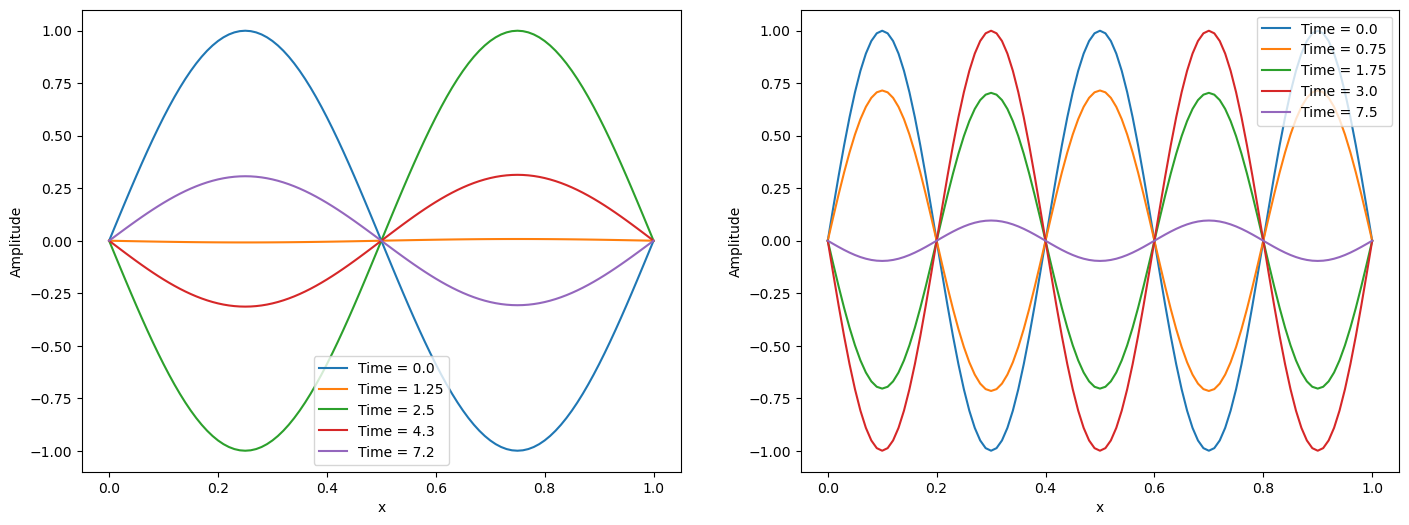
\includegraphics[width = 0.6\textwidth]{Images/qc_1.png}
        \caption{Binomial tree convergence}
        \label{fig:qc1}
    \end{center}
\end{figure}


As can be observed in \ref{fig:qc_1}, both wqave behave similaryly. With the first case
a) resulting in two constant interchangable peaks, due double to the multiplicty of the $sin(x)$ function.
In contrast, the second case observes afive intercahngeble peaks for the same reasons($\psi(x, t= 0) = sin(5\pi x)$).
Laslty, note thatm in birh cases the peaks are interchanged at every 1 second, this result is due our inttial conditons,
where the speed of propagation $c$ set at 1 second.

For the third case, the wave is set at





This concludes our test LaTeX document.

\end{document}
